\subsubsection*{UMap}

\paragraph{Overview}

UMap is a user level library providing a high performance mmap-like
interface that can be tuned to application needs without requiring OS
customization or impacting system configuration. UMap enables
applications to interact with out-of-core data sets as if in memory,
and to configure parameters such as page buffer size and page size on
a per-application basis.

Leadership supercomputers feature a diversity of storage, from
node-local persistent memory and NVMe SSDs to network-interconnected
flash memory and HDD. Interacting with large persistent data sources
is critical to exascale applications that harness the power of data
analytics and machine learning. The UMap user-level library enables
user-space page management of data located in the memory/storage
hierarchy. By providing a memory map interface, applications can
interact with large data sets as if in memory. As a user level
library, a UMap page fault handler can be easily adapted to access
patterns in applications and to storage characteristics, reducing latency
and improving performance.

\paragraph{Key Challenges}

As ECP applications transition to include ML and data analytics as
integral components of workflows, persistent memories and low latency
storage devices offer new alternatives to hold portions of very large
global data sets within the fabric of the computing system. These new
applications drive new access patterns, i.e. read-dominated analysis
of observational or simulation data rather than write-mostly
checkpoints. The combination of new technologies (byte addressable,
very low latency, asymmetric read/write latency), new insertion points
(node local, Top of Rack or other intermediate storage, global FS,
external distributed storage servers), and new applications (in-situ
analytics, experimental $+$ simulation data analysis, ML batched data
sets) present challenges both to the traditional memory/storage
dichotomy as well as to traditional HPC I/O libraries tailored to
checkpoint transmission.

\paragraph{Solution Strategy}

We prioritize four design choices for UMap based on surveying
realistic use cases. First, we choose to implement UMap as a
user-level library so that it can maintain compatibility with the
fast-moving Linux kernel without the need to track and modify for
frequent kernel updates. Also, we employ the recent userfaultfd 
mechanism, rather than the signal handling + callback function approach
to reduce overhead and performance variance in multi-threaded
applications. Third, we target an adaptive solution that sustains
performance even at high concurrency for data-intensive applications,
which often employ a large number of threads for hiding data access
latency. Our design pays particular consideration on load imbalance
among service threads to improve the utilization of shared resources
even when data accesses to pages are skewed. UMap dynamically balances
workloads among all service threads to eliminate bottleneck on serving
hot pages. Finally, for flexible and portable tuning on different
computing systems, UMap provides both API and environmental controls
to enable configurable page sizes, eviction strategy, application-
specific prefetching, and detailed diagnosis information to the
programmer. The UMap software architecture is shown in Figure
\ref{fig:umaparch}.

\begin{figure}[t]
        \centering
        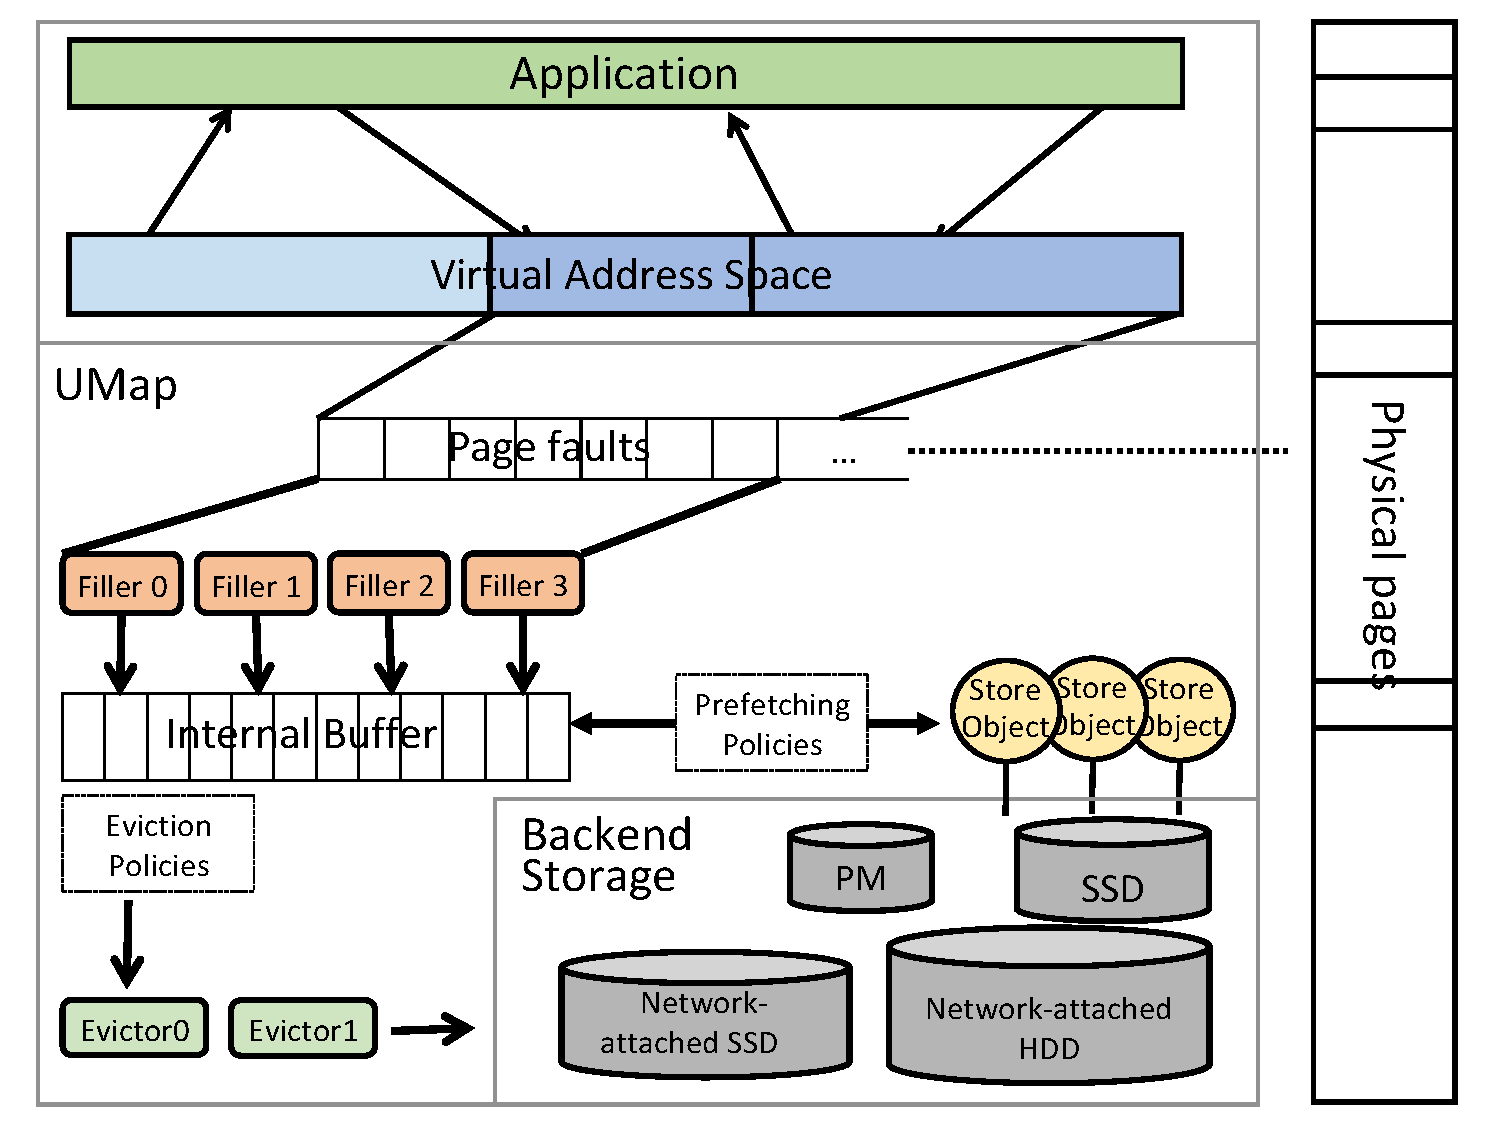
\includegraphics[scale = 0.5]{projects/2.3.1-PMR/2.3.1.19-Argo-PowerSteering/umap-arch}
        \caption{UMap Handler architecture}
        \label{fig:umaparch}
\end{figure}

\paragraph{Recent Progress}

In recent months, we have released UMap v. 2.0, with major
enhancements to improve load balancing and incorporate features for
additional configurability. We have used UMap in new applications
including a key/value store and the lrzip utility.

A paper on UMap will be presented at the Memory Centric HPC Workshop
(MCHPC) at SC19.

\paragraph{Next Steps}
In the coming year we plan to continue outreach to application teams
within ECP and in the science/data community. We plan to implement a
new UMap handler for the persistent memory Meta Allocator (Metall)
which is part of SICM. Metall provides support for persistent heaps as
an alternative to data serialization, and is being considered for use by the
Exagraph and EXAALT code teams. We plan to add support for
disaggregated in-system memory/storage in the core UMap handler to
augment the existing file-backed mechanism. This will enable
applications to access data on other nodes in the network without
requiring explicit remote file system mount points on each node.
